\pagebreak

%%%%%%%%%%%%%%%%%%%%%%%%%%%%%%%%%%%%%%%%


\section{Allgemeines}

\section{Produktübersicht}

\section{Grundsätzliche Struktur- und Entwurfsprinzipien}

Die Grundsätzliche Struktur des GSB ist im Komponentendiagramm
(Abb. \ref{fig02}) schematisch dargestellt.

%\begin{SCfigure}[20][htbp]%
\begin{figure}[h]%
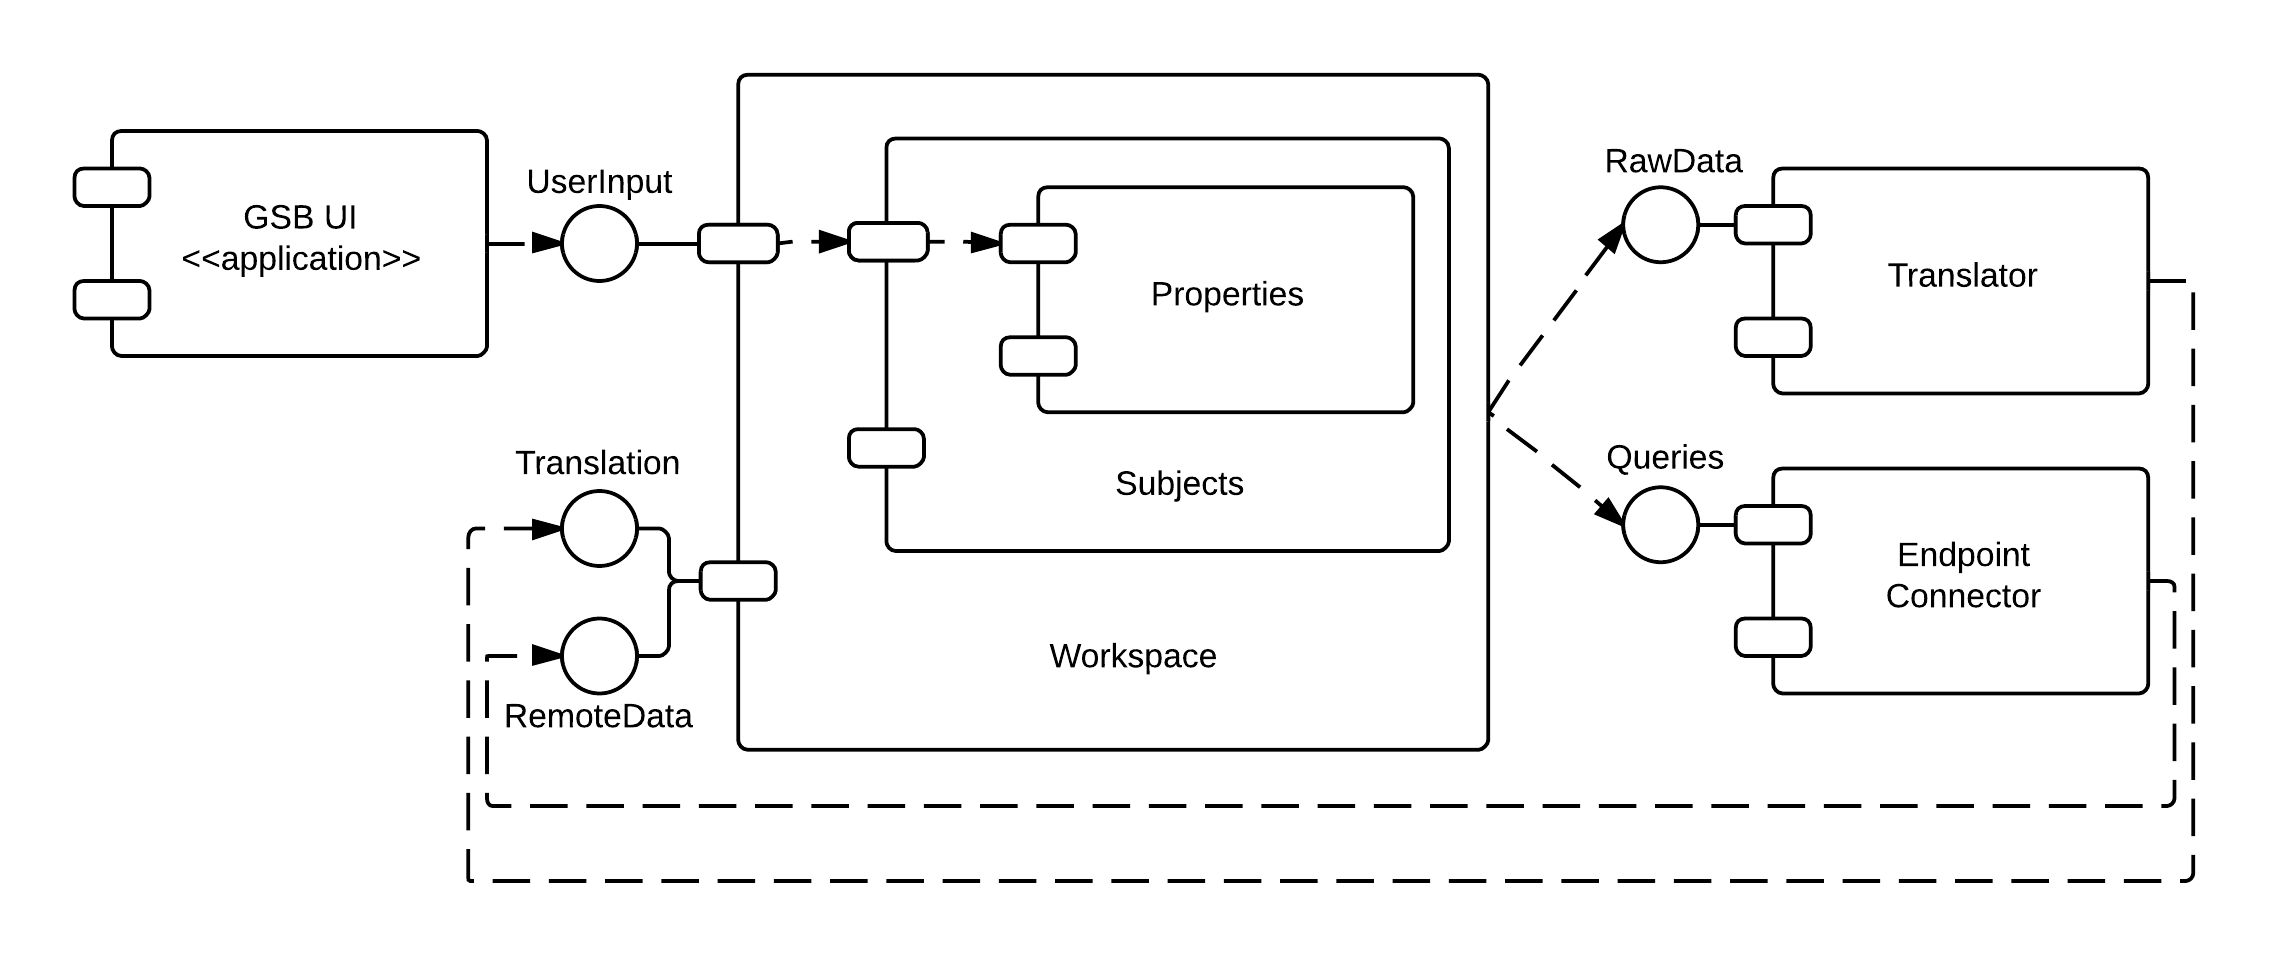
\includegraphics[width=\hsize]{Komponentendiagramm.png}
\caption{Komponentendiagramm des GSB.}
\label{fig02}
\end{figure}
%\end{SCfigure}


Es gibt die Komponente des User Interface (GSB UI), in welcher alle
Eingaben des Benutzers des Tools stattfinden. Diese werden in die
Komponente Workspace weitergeleitet und dort gegebenenfalls an die
Komponenten Subjects und deren Unterkomponente Properties
weitergeleitet. Um dies zu verdeutlichen, hier drei Beispiele:
\begin{enumerate}
\item Der Nutzer setzt eine Übersetzung eines GSBL-Wortes in Gang, dies betrifft die Komponente “Workspace”
\item Der Nutzer ändert den Alias eines Subjekts, dies würde über die Workspace-Komponente zu der Subjects-Komponente weitergereicht werden.
\item Der Nutzer ändert die Sichtbarkeit einer Eigenschaft, dies würde über die Workspace-Komponente zu der Subjects-Komponente zum Ziel, der Properties-Komponente, weitergereicht werden.
\end{enumerate}
Die Workspace-Komponente steht in Verbindung mit der
Translator-Komponente, welche für die Übersetzung der erstellten
Rohdaten zu JSON bzw. SPARQL zuständig ist und die Ergebnisse zurück
zur Workspace-Komponente überträgt.
Ebenso gibt es eine Verbindung zur Endpoint-Connector-Komponente, die die Kommunikation mit einem Endpoint übernimmt. Es können Anfragen gesendet und Ergebnisse empfangen werden.



\section{Struktur- und Entwurfsprinzipien einzelner Pakete}

\section{Datenmodell}

\section{Testkonzept}

%%% Local Variables: 
%%% mode: latex
%%% TeX-master: "main"
%%% End: 
